\documentclass{article}
\usepackage[a4paper, margin=1in]{geometry}
\usepackage[utf8]{inputenc}
\usepackage[T1]{fontenc}
\usepackage{lmodern}
\usepackage{amsmath, amssymb, graphicx, hyperref}
\graphicspath{{../figures/}}
\usepackage[framed,numbered]{matlab-prettifier}
\usepackage{xcolor}
\usepackage{bookmark}
\usepackage{listings}

\geometry{a4paper, margin=1in}

% MATLAB code style
\lstset{
  style      = Matlab-editor,
  basicstyle = \mlttfamily,
  breaklines = true
}

\title{\textbf{Practical - 4}}
\author{}
\date{October 10, 2026}

\pagenumbering{gobble}

\begin{document}
\maketitle

\noindent
\textbf{\large{Aim:}} To solve system of equations.

\vspace{1em}
\noindent
\textbf{\large{Theory:}}

\vspace{0.5em}
\noindent
\textbf{1. What is a system of ODEs?}

\noindent
Till now, we solved one differential equation, for example:
\[\frac{dy}{dt} = f(t, y)\]
Now we have two differential equations involving two unknown functions:
\begin{equation*}
  \boxed{
    \begin{aligned}
      \frac{dx}{dt} &= f(t, x, y) \\
      \frac{dy}{dt} &= g(t, x, y).
    \end{aligned}
  }
\end{equation*}

\begin{center}
  \rule{1.0\textwidth}{0.4pt}
\end{center}

\noindent
For Example

\noindent
take the system
\[\frac{dx}{dt} = x + y\]
\[\frac{dy}{dt} = x - y\]
with initial conditions
\[x(0) = 1, \quad y(0) = 0\]

\vspace{1em}
\noindent
\textbf{\large{MATLAB Code:}}
\begin{lstlisting}
clc; clear all; close all;

syms x(t) y(t)

eqn1 = diff(x,t) == x+y;
eqn2 = diff(y,t) == x-y;

init1 = x(0) == 1;
init2 = y(0) == 0;

[xSol,ySol] = dsolve([eqn1, eqn2],[init1, init2]); %%%Solve both differential equations simultaneously subject to both initial conditions.

disp('Solution for x(t):')
disp(xSol)

disp('Solution for y(t):')
disp(ySol)

fplot(xSol, [0 5], 'LineWidth', 2)
hold on
fplot(ySol, [0 5], 'LineWidth', 2)

grid on
xlabel('Time t')
ylabel('Solution')
title('Solution of system of ODEs')
legend('x(t)','y(t)')
hold off
\end{lstlisting}

\vspace{1em}
\noindent
\textbf{\large{Output:}}
\begin{flushleft}
\tiny{Solution for x(t):}
\end{flushleft}
\begin{flushleft}
$\frac{\sqrt{2}\,{\mathrm{e}}^{\sqrt{2}\,t} \,{\left(\sqrt{2}+1\right)}}{4}+\frac{\sqrt{2}\,{\mathrm{e}}^{-\sqrt{2}\,t} \,{\left(\sqrt{2}-1\right)}}{4}$
\end{flushleft}
\begin{flushleft}
\tiny{Solution for y(t):}
\end{flushleft}
\begin{flushleft}
$\frac{\sqrt{2}\,{\mathrm{e}}^{\sqrt{2}\,t} }{4}-\frac{\sqrt{2}\,{\mathrm{e}}^{-\sqrt{2}\,t} }{4}$
\end{flushleft}
\begin{figure}[htbp]
    \centering
    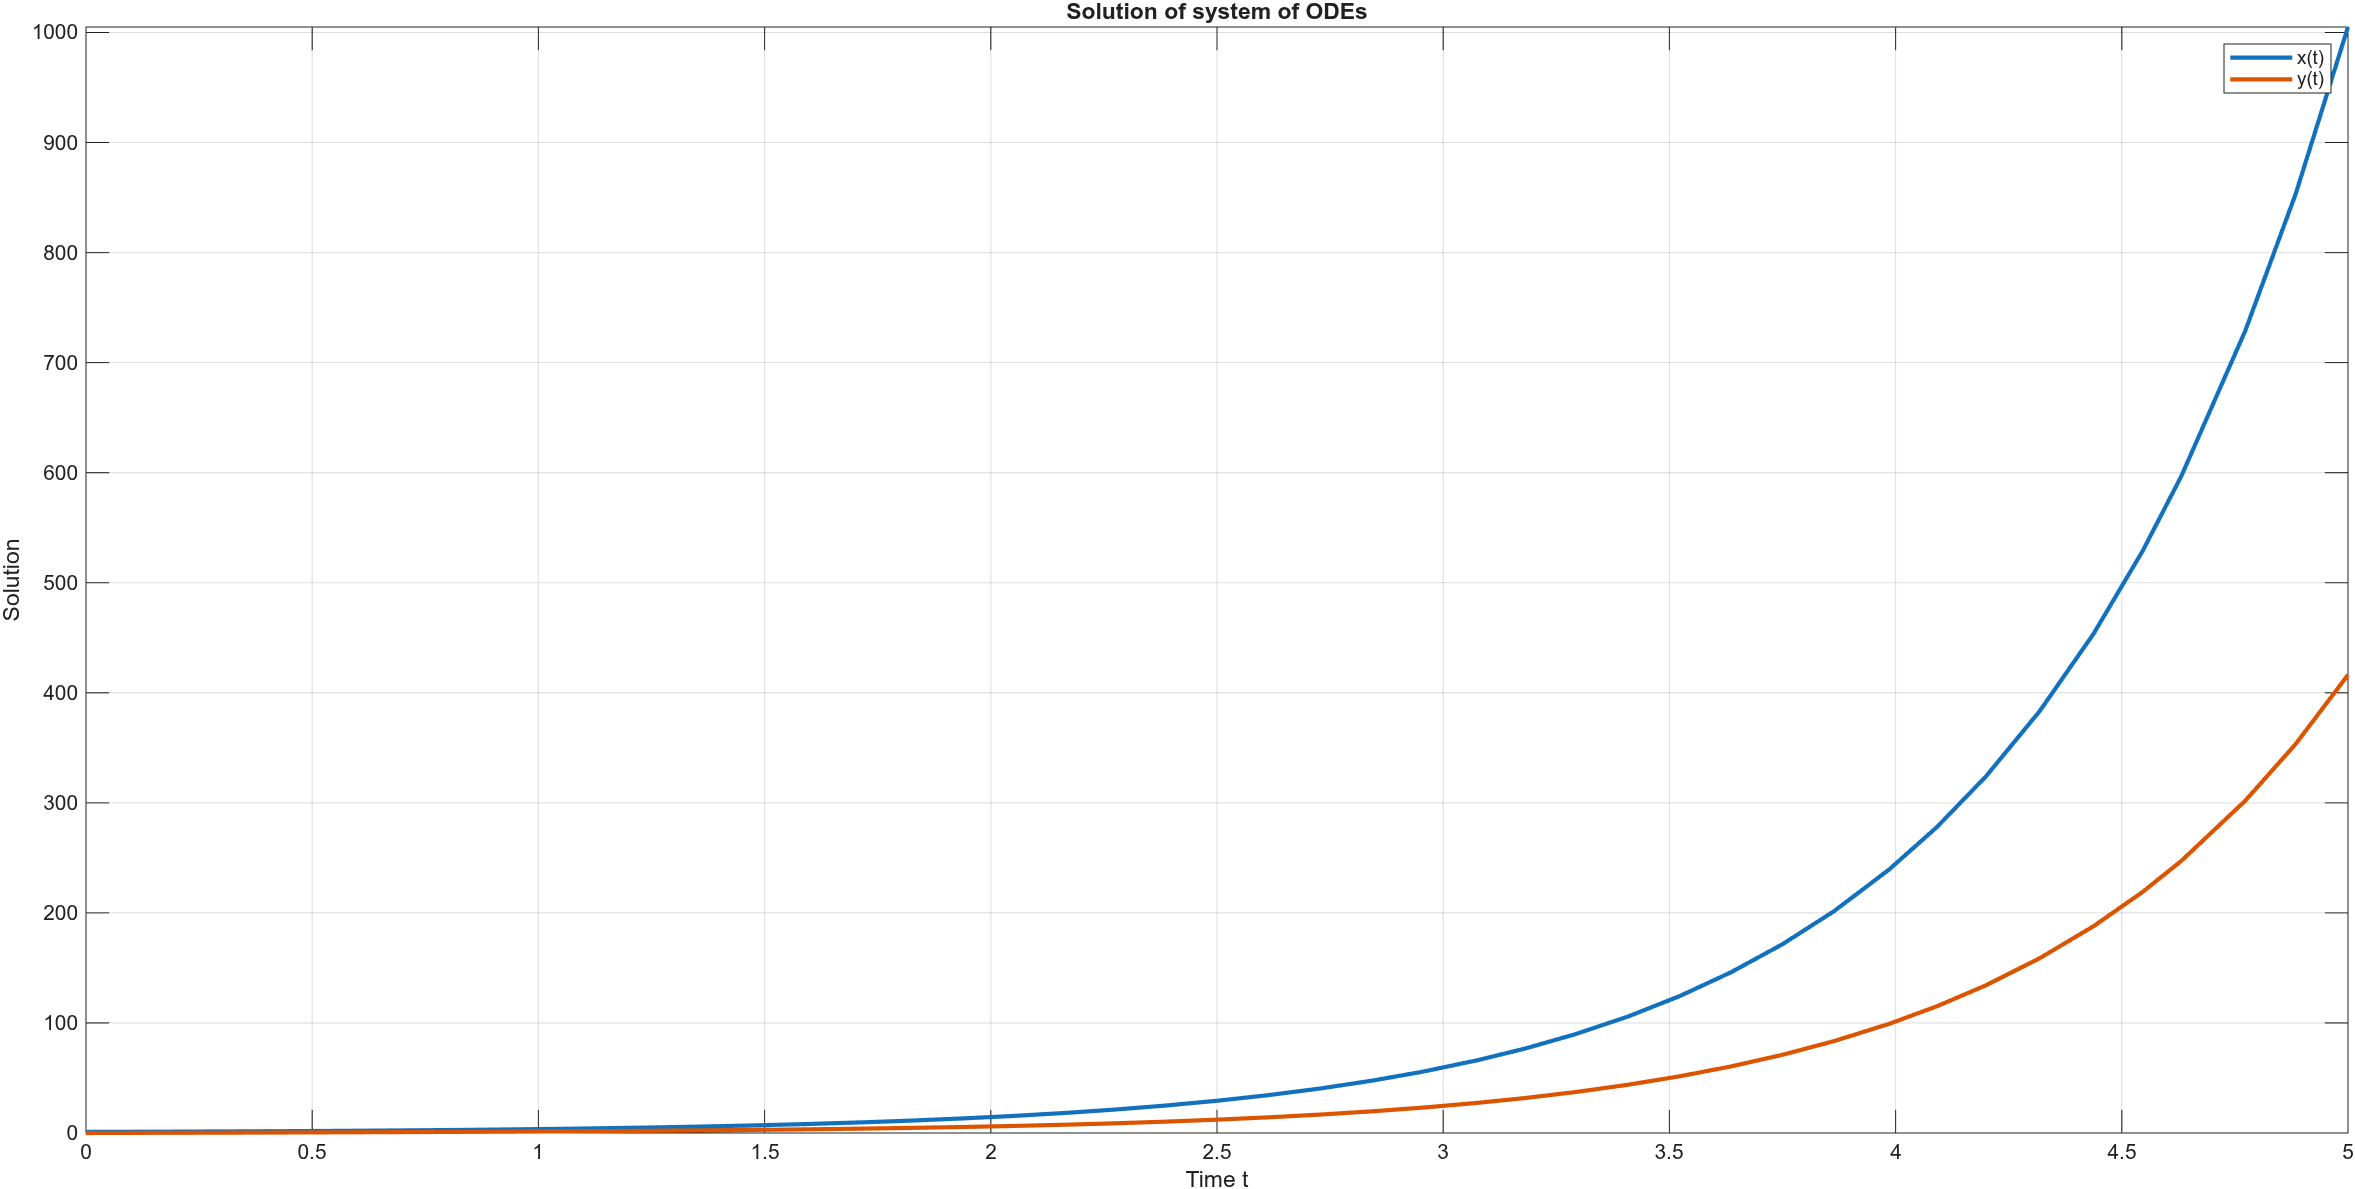
\includegraphics[width=0.7\textwidth]{Figure4.png}
\end{figure}

\end{document}
